\documentclass[tikz,border=10pt]{standalone}

\usepackage{tikz}
\usetikzlibrary{positioning,fit,calc,shapes.geometric}

\begin{document}

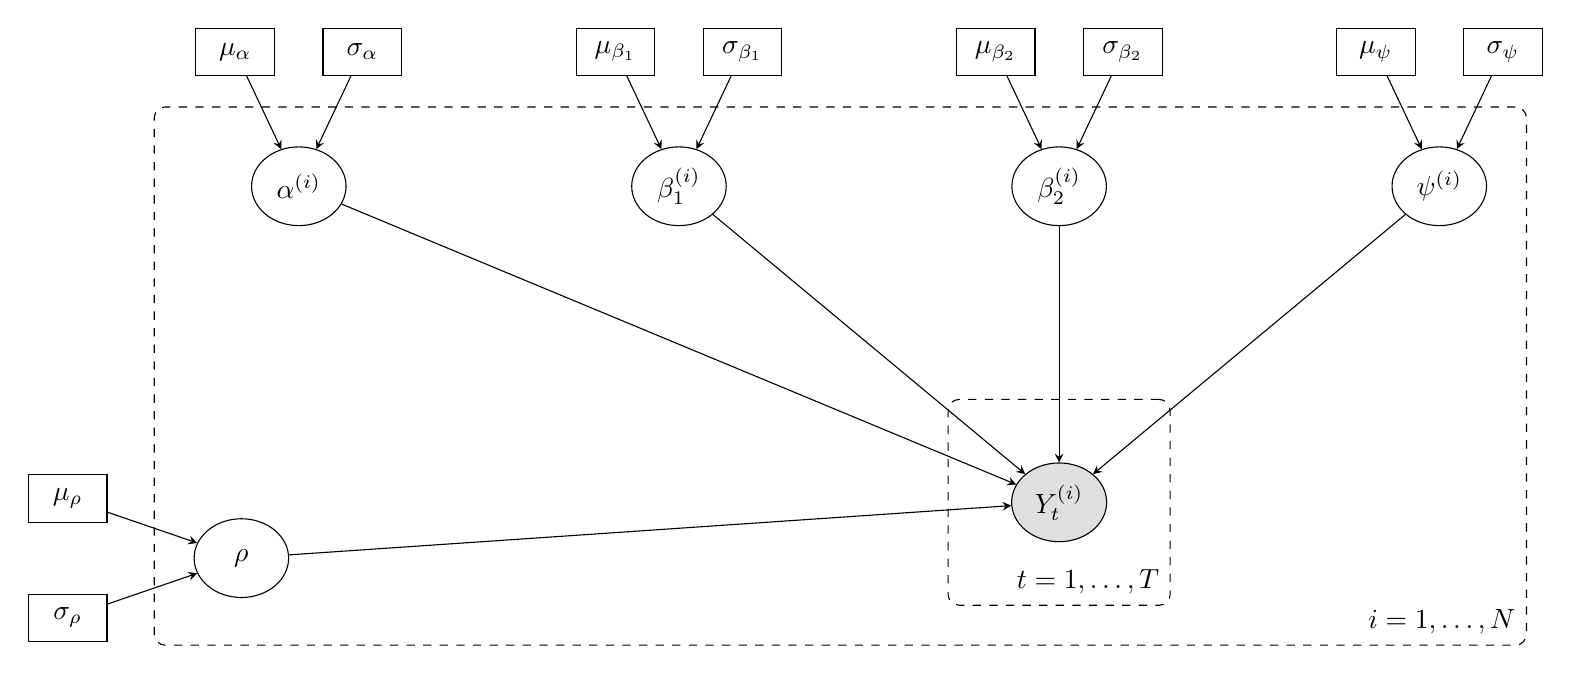
\begin{tikzpicture}[
    >=stealth,
    latent/.style={
        draw,
        shape=ellipse,
        minimum width=1.2cm,
        minimum height=1cm
    },
    hyper/.style={
        draw,
        rectangle,
        minimum width=1.0cm,
        minimum height=0.6cm
    },
    plate/.style={
        draw,
        dashed,
        rounded corners,
        inner sep=0.5cm
    }
]

%%%%%%%%%%%%%%%%%%%%%%%%%%%%%%%%%%%%%%%%%%%%%%%%%%%%
%% Hyperparameters
%%%%%%%%%%%%%%%%%%%%%%%%%%%%%%%%%%%%%%%%%%%%%%%%%%%%

\node[hyper] (mua) {$\mu_\alpha$};
\node[hyper,right=0.6cm of mua] (sa) {$\sigma_\alpha$};

\node[hyper,right=2.2cm of sa] (mubone) {$\mu_{\beta_1}$};
\node[hyper,right=0.6cm of mubone] (sbone) {$\sigma_{\beta_1}$};

\node[hyper,right=2.2cm of sbone] (mubtwo) {$\mu_{\beta_2}$};
\node[hyper,right=0.6cm of mubtwo] (sbtwo) {$\sigma_{\beta_2}$};

\node[hyper,right=2.2cm of sbtwo] (mupsi) {$\mu_\psi$};
\node[hyper,right=0.6cm of mupsi] (spsi) {$\sigma_\psi$};

%%%%%%%%%%%%%%%%%%%%%%%%%%%%%%%%%%%%%%%%%%%%%%%%%%%%
%% Coordinates for centered placement
%%%%%%%%%%%%%%%%%%%%%%%%%%%%%%%%%%%%%%%%%%%%%%%%%%%%

\coordinate (alphamid)   at ($(mua)!0.5!(sa)$);
\coordinate (betaonemid) at ($(mubone)!0.5!(sbone)$);
\coordinate (betatwomid) at ($(mubtwo)!0.5!(sbtwo)$);
\coordinate (psimid)      at ($(mupsi)!0.5!(spsi)$);

%%%%%%%%%%%%%%%%%%%%%%%%%%%%%%%%%%%%%%%%%%%%%%%%%%%%
%% Individual-level parameters
%%%%%%%%%%%%%%%%%%%%%%%%%%%%%%%%%%%%%%%%%%%%%%%%%%%%

\node[latent,below=1.2cm of alphamid] (alpha)
{$\alpha^{(i)}$};

\node[latent,below=1.2cm of betaonemid] (betaone)
{$\beta_1^{(i)}$};

\node[latent,below=1.2cm of betatwomid] (betatwo)
{$\beta_2^{(i)}$};

\node[latent,below=1.2cm of psimid] (psi)
{$\psi^{(i)}$};

%%%%%%%%%%%%%%%%%%%%%%%%%%%%%%%%%%%%%%%%%%%%%%%%%%%%
%% Observation
%%%%%%%%%%%%%%%%%%%%%%%%%%%%%%%%%%%%%%%%%%%%%%%%%%%%

\node[
    latent,
    fill=gray!25,
    below=3cm of betatwo
] (y)
{$Y_t^{(i)}$};

%%%%%%%%%%%%%%%%%%%%%%%%%%%%%%%%%%%%%%%%%%%%%%%%%%%%
%% Hyperparameter arrows
%%%%%%%%%%%%%%%%%%%%%%%%%%%%%%%%%%%%%%%%%%%%%%%%%%%%

\draw[->] (mua) -- (alpha);
\draw[->] (sa) -- (alpha);

\draw[->] (mubone) -- (betaone);
\draw[->] (sbone) -- (betaone);

\draw[->] (mubtwo) -- (betatwo);
\draw[->] (sbtwo) -- (betatwo);

\draw[->] (mupsi) -- (psi);
\draw[->] (spsi) -- (psi);

%%%%%%%%%%%%%%%%%%%%%%%%%%%%%%%%%%%%%%%%%%%%%%%%%%%%
%% Observation arrows
%%%%%%%%%%%%%%%%%%%%%%%%%%%%%%%%%%%%%%%%%%%%%%%%%%%%

\draw[->] (alpha) -- (y);
\draw[->] (betaone) -- (y);
\draw[->] (betatwo) -- (y);
\draw[->] (psi) -- (y);

%%%%%%%%%%%%%%%%%%%%%%%%%%%%%%%%%%%%%%%%%%%%%%%%%%%%
%% rho
%%%%%%%%%%%%%%%%%%%%%%%%%%%%%%%%%%%%%%%%%%%%%%%%%%%%

\node[hyper,below left=3.3cm and 2cm of alpha] (murho)
{$\mu_\rho$};

\node[hyper,below=0.9cm of murho] (srho)
{$\sigma_\rho$};

\coordinate (rhomid) at ($(murho)!0.5!(srho)$);

\node[latent,right=1.6cm of rhomid] (rho)
{$\rho$};

\draw[->] (murho) -- (rho);
\draw[->] (srho) -- (rho);
\draw[->] (rho) -- (y);

%%%%%%%%%%%%%%%%%%%%%%%%%%%%%%%%%%%%%%%%%%%%%%%%%%%%
%% Plates
%%%%%%%%%%%%%%%%%%%%%%%%%%%%%%%%%%%%%%%%%%%%%%%%%%%%

\node[
    plate,
    fit=(y),
    inner xsep=0.8cm,
    inner ysep=0.8cm
] (timeplate) {};

\node[
    anchor=south east,
    inner sep=2pt
] at ($(timeplate.south east)+(-2pt,2pt)$)
{$t=1,\ldots,T$};

\node[
    plate,
    fit=(alpha)(betaone)(betatwo)(psi)(rho)
        (timeplate)
] (subjectplate) {};

\node[
    anchor=south east,
    inner sep=2pt
] at ($(subjectplate.south east)+(-2pt,2pt)$)
{$i=1,\ldots,N$};

\end{tikzpicture}

\end{document}